%% Lezione di esempio. Copiate questo file nella lezione che dovete creare
%% per avere già uno scheletro di come scrivere le lezioni

%% Diamo un nome al capitolo. Idealmente mettiamo la data della lezione ed
%% una sua breve descrizione / argomenti trattati
\chapter{24 Ottobre 2016 - Teorema di Picard e biolomorfismi di tori}
\justify

Si prosegue con le notazioni della scorsa lezione.
Nelle scorsa lezioni si è visto che è possibile classificare le Superfici di Riemann come quozienti di:
\begin{enumerate}
\item $\mathbb{P}^1(\mathbb{C})=\hat{\bbC}$
\item $\bbC$
\item $\mathbb{D} \cong \mathcal{H}$
\end{enumerate}
per un gruppo $G\le\Aut(\tilde{X})$ di automorfismi che agisce in maniera propriamente discontinua e senza punti fissi.

Ne segue che per classificare le superfici di Riemann è sufficiente classificare i sottogruppi dei gruppi di automorfismi della superfici $1)$, $2)$ e $3)$.

\newthought{Caso 1, Sferica.} Si è visto nella scorsa lezione che c'è una sola superficie di Riemann di questo tipo ed è $\hat{\bbC}$.

\newthought{Caso 2, Euclidea.} Si è visto nella scorsa lezione che i sottogruppi $G\le\Aut(\tilde{X})=Aff(\bbC)$ del tipo che si cerca sono dei reticoli $L$ di rango che può essere solo $0$,$1$ o $2$. Distinguiamo quindi tre casi:
\begin{itemize}
\item $\Rk L=0$, l'unica superficie di Riemann è $\bbC$.
\item $\Rk L=1$, l'unica superficie di Riemann è $\quotient{\bbC}{L}$, in cui siccome $L$ ha rango uno si ha $L=\omega \bbZ$, con $\omega\in\bbC$ non nullo. Quindi eseguendo un'omotetia di parametro $\omega$ (è un biolomorfismo) si ha che $X\cong \quotient{\bbC}{\bbZ}$.
Osserviamo che in questo caso si ha che $\quotient{\bbC}{\bbZ}\cong \bbC^{*}=\mathbb{P}^1(\mathbb{C})\minus\{0,\infty\}$ tramite la mappa esponenziale, e che $\bbC^{*}=\mathbb{G}_m(\bbC)$, il gruppo algebrico moltiplicativo di $\bbC$. Quindi si possono trasferire le operazioni di gruppo di $\bbC^{*}$ su $\quotient{\bbC}{\bbZ}$ tramite la mappa esponenziale, cosa che si farà più avanti in modo analogo con le curve algebriche.
\item $\Rk L=2$, in questo caso si hanno i Tori, $\quotient{\bbC}{L}$ con $L$ reticolo di rango $2$, che si studieranno più avanti in questa lezione.
\end{itemize}
\newthought{Caso 3, Iperbolica.} Ci sono molti problemi aperti...

\notamargine{Se una superficie di Riemann non è né Sferica né Euclidea allora è Iperbolica.}

\begin{osservazione}
Nel caso di Superficie di Riemann Sferica e nei tre casi di Superficie di Riemann Euclidea si sa calcolare il gruppo fondamentale ($\pi_1$). (è il gruppo per cui si quozienta)
\end{osservazione}

\begin{esercizio}
Sia $A$ un dominio (aperto connesso) limitato di $\bbC$. Si dimostri che se si considera su $A$ la struttura di superficie di Riemann indotta dalla mappa di inclusione $A\hrar\bbC$ allora $A$ è una superficie di Riemann iperbolica.
\end{esercizio}


\notamargine{Può essere utile utilizzare un ragionamento per esclusione.}

\begin{esercizio}Sia $S=\mathbb{P}^1(\mathbb{C})\minus\{0,1,\infty\}$, si dimostri che se si considera la struttura di superficie di Riemann indotta dalla mappa di inclusione $S\hrar\mathbb{P}^1(\mathbb{C})$ allora $S$ è una superficie di Riemann iperbolica.
\end{esercizio}

\notamargine{Essendo $\mathbb{P}^1(\mathbb{C})$ triplamente transitivo in realtà si sarebbe potuto scegliere $\mathbb{P}^1(\mathbb{C})\minus\{ A, B, C\}$, con $\{ A, B, C\}$ tre punti distinti di $\mathbb{P}^1(\mathbb{C})$.}

\begin{proof}Lo si dimostrerà in tre modi.
\begin{itemize}
\item Il gruppo fondamentale di $S$ è isomorfo al prodotto libero di due copie di $\bbZ$ quindi non è abeliano. Si escludono perciò i casi di Superficie di Riemann Sferica e Euclidea, perché in quei casi il gruppo fondamentale è abeliano.
\item Si escluderanno i casi di Superficie di Riemann Sferica e Euclidea. $S$ non è compatta, quindi non puù essere biolomorfa alla Sfera di Riemann e nemmeno ad un toro $\quotient{\bbC}{L}$ con $L$ reticolo di rango $2$. Rimangono da escludere i casi $\quotient{\bbC}{\bbZ}$ e $\bbC$.\\
Si esclude il caso $\quotient{\bbC}{\bbZ}={\bbC}^*$:\\
Si osserva che $S=\bbC^*\minus\{ 1\}\subset\bbC$, quindi se esistesse $f:\bbC^*\rightarrow\bbC^*\minus\{ 1\}\subset\bbC$ olomorfa e iniettiva allora $f$ non potrebbe avere una singolarità essenziale né in $0$ né in $\infty$.\\
Infatti $f$ è aperta perciò se si prende un disco aperto $D$ in $\bbC^*$ si ha che la sua immagine è un aperto di $\bbC$. Se per assurdo $f$ avesse una singolarità essenziale in $0$ allora per il Teorema di Weierstrass ogni intorno bucato di $0$ avrebbe immagine densa in $\bbC$ quindi in particolare considerando un intorno bucato di $0$ disgiunto da $D$ si ha che un punto dell'intorno bucato andrebbe in $f(D)$, contraddicendo l'iniettività della mappa $f$. Con lo stesso ragionamento si trova che $f$ non può avere una singolarità essenziale all'infinito.\\
Quindi non avendo singolarità essenziali né in $0$ né in $\infty$ può essere estesa ad una mappa meromorfa con dominio tutto $\mathbb{P}^1(\mathbb{C})$, ne segue che è una mappa razionale (nello $0$ ha al più un polo, quindi $\exists n\in\mathbb{N} \quad z^nf$ è olomorfa in $\bbC$, ne segue che $z^nf$ ha al più un polo all'infinito quindi è un polinomio, quindi $f$ è razionale) e che quindi siccome $f$ ristretta a $\bbC^*$ deve essere iniettiva deve essere quoziente di due polinomi lineari (sennò fissato $a\in\bbC$ si ha che $f(z)=\frac{(z-\alpha_1)\cdots (z-\alpha_k)}{z^n}=a$ ha più di una soluzione). Quindi $f$ si deve estendere ad un automorfismo di $\mathbb{P}^1(\mathbb{C})$, altrimenti se $f$ si estendesse a $\frac{az+b}{cz+d}$ con $ad-bc=0$ si avrebbe che $\frac{az+b}{cz+d}=\frac{b\frac{c}{d} z+b}{cz+d}=\frac{b}{d} \frac{cz+d}{cz+d}=\frac{b}{d}$ quindi non sarebbe iniettiva. Ma se $f$ si estende ad un automorfismo di $\mathbb{P}^1(\mathbb{C})$ si ha che, siccome alla $f$ iniziale si sono aggiunti $2$ punti, non può essere che l'immagine sia surgettiva, quindi a meno di scegliere la carta con il punto mancante all'infinito si ha che l'immagine è un compatto di $\bbC$ quindi che $f$ è limitata quindi costante.
Si esclude il caso $\bbC$ con lo stesso ragionamento del punto precedente.

\item $S$ ha la proprietà $\mathcal{P}:= $ $\exists K$ compatto t.c.$\forall K'$ compatto con $K\subseteq K'\subseteq S$ vale che $S\minus K'$ ha almeno $3$ componenti connesse.
Sia $K$ un compatto di $\mathbb{P}^1(\mathbb{C})\minus\{ A, B, C\}$, che è quindi un compatto di $\mathbb{P}^1(\mathbb{C})$. Quest'ultimo è $T2$ quindi $K$ è chiuso in $\mathbb{P}^1(\mathbb{C})$, quindi il complementare è aperto. Allora si ha che si riescono a trovare dei dischi aperti di $\mathbb{P}^1(\mathbb{C})$ attorno ai punti $A, B, C$ che non intersecano il compatto.

\begin{figure}[h]
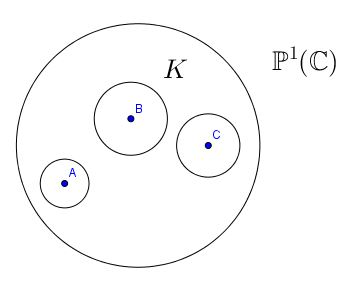
\includegraphics[width=5.7cm]{lezione-161024-fig1}
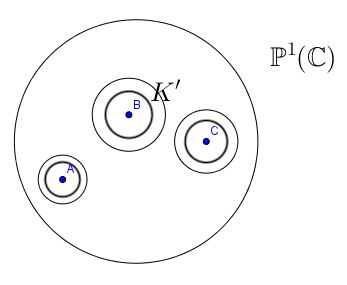
\includegraphics[width=6cm]{lezione-161024-fig2}
\caption{$K$ e $K'$}\label{fig:1}
\end{figure}

Quindi se $A, B, C$ sono i punti che si tolgono da $\mathbb{P}^1(\mathbb{C})$, allora si può scegliere $K'$ come $\mathbb{P}^1(\mathbb{C})\minus\{D_A\cup D_B\cup D_C\}$, con $D_A$ disco aperto attorno a $A$, $D_B$ disco aperto attorno a $B$, $D_C$ disco aperto attorno a $C$, perciò la proprietà.\\
Si osserva che la proprietà $\mathcal{P}$ è invariante per omeomorfismi quindi in particolare per biolomorfismi e che quindi non essendo soddisfatta dalle superfici di Riemann Sferica e Euclidee ne segue che $S$ è iperbolica.
Infatti si ha che si escludono le superfici compatte prendendo come $K'$ loro stesse, si esclude $\bbC$ prendendo come $K'$ il complementare di un disco aperto che contiene $K$ e si esclude $C^*=\mathbb{P}^1(\mathbb{C})\minus\{ 0,\infty\}$ perché con il ragionamento fatto per dimostrare la proprietà $\mathcal{P}$ su $S$ si dimostra che si trovano dei compatti $K'$ con $2$ componenti connesse, quindi non $almeno\hquad 3$, come richiesto dalla proprietà.
\end{itemize}
\end{proof}

\notamargine{La proprietà $\mathcal{P}$ in un qualche senso "conta i punti tolti, in funzione di quello che è rimasto". Inoltre permette di dire per esempio che un "toro meno $n$ punti distinti" non è omeomorfo a un "toro meno $m$ punti distinti", se $m\ne n$}

\begin{teorema}[Teorema di Picard]
Ogni funzione intera ($\bbC\rightarrow\bbC$ olomorfa su tutto $\bbC$) non costante assume tutti i valori tranne al più uno.
\end{teorema}

\begin{osservazione}
\begin{itemize}
\item La mappa esponenziale assume tutti i valori tranne lo $0$
\item Se la mappa $f$ come da ipotesi ha in più la proprietà di NON avere una discontinuità essenziale all'infinito allora si ha che per Liouville deve essere un polinomio, quindi il risultato è banale ($p(x)-a$ ha sempre almeno una radice, se $p$ non costante)
\end{itemize}
\end{osservazione}

\notamargine{C'è anche una versione più forte di questo teorema (detto da lui)}

\begin{proof}
Si usa che $\mathbb{P}^1(\mathbb{C})\minus\{ A, B, C\}$ con $A, B, C$ tre punti distinti è una superficie di Riemann iperbolica (Esercizio 7).\\
Si suppone per assurdo che $f$ soddisfacente le ipotesi non assuma due valori, che a meno di comporre $f$ con un'affinità (automorfismo di $\bbC$) suppongo essere $0,1$.
Allora $f$ induce una mappa olomorfa $f:\bbC->S$ (con $S$ come in Esercizio 7).
Si ha che quindi $f$ si solleva a $\tilde{f}:\bbC\rightarrow D$, con $D$ il disco aperto. DIAGRAMMA \\
Ma allora la mappa olomorfa $\tilde{f}$ è costante per Liouville, quindi poiché il diagramma commuta anche $f$ è costante, assurdo.
\end{proof}

\begin{osservazione}
\begin{itemize}
\item Questo è un teorema non di facile dimostrazione, il punto più delicato nella dimostrazione data è il teorema di Riemann.
\item Nella dimostrazione data il teorema di Riemann serve per l'esistenza di un rivestimento $\pi:D\cong \mathcal{H} \rightarrow S$. In effetti si può dimostrare il teorema di Picard esibendo un rivestimento, Picard face proprio così. Trovò il rivestimento quozientando $\mathcal{H}$ per il gruppo $\Gamma(2)=\{ \frac{az+b}{cz+d} | a,b,c,d\in \bbZ, ad-bc=1, a\cong d \cong 1 \pmod{2}, b\cong c \cong 0 \pmod{2} \}$, dopo aver dimostrato che questo gruppo agiste su $\mathcal{H}$ con le proprietà viste nelle scorse lezioni poiché effettivamente il quoziente sia una superficie di Riemann ed aver verificato che il quoziente è $S$.
\item Ci sono molte altre dimostrazioni con tecniche più analitiche, quella che si è fatta è più geometrica, senza stime. 
\end{itemize}
\end{osservazione}

\section{Biolomorfismi di tori}
D'ora in poi non ci si interessa più di superfici di Riemann iperboliche ma si iniziano a studiare i Tori, ovvero quozienti $\quotient{\bbC}{L}$ con $L$ reticolo di rango $2$.

\notamargine{Attenzione, molti matematici usano nella definizione di reticolo il fatto che il reticolo abbia la stessa dimensione dello spazio vettoriale in cui è contenuto, nel nostro caso è contenuto in $\bbC$ che ha dimensione reale $2$.}

\begin{osservazione}
Se prendiamo reticoli omotetici, ovvero due reticoli $L$ e $\lambda L$, con $\lambda \in \bbC\minus\{ 0\}$, si ha che i tori ottenuti sono biolomorfi. (La mappa moltiplicazione per $\lambda \quad \bbC \rightarrow \quotient{\bbC}{\lambda L} \hquad z\ \mapsto [\lambda z]_{\lambda L} $ è ben definita e passa al quoziente $\quotient{\bbC}{L}\rightarrow \quotient{\bbC}{\lambda L}$, che è olomorfa e ha come inversa olomorfa la moltiplicazione per $\lambda^{(-1)}$).
\end{osservazione}

\begin{fatto}Sia $f:T_1\rightarrow T_2$ olomorfa tra tori, con $T_i=\quotient{\bbC}{L_i},\hquad i\in \{ 1,2\}$, allora $\exists\alpha \hquad \alpha L_1\subseteq L_2$.\\
(CON ALPHA UGUALE A $0$ FUNZIONA SEMPRE, PROBABILMENTE INTENDE CHE SE $f$ NON NULLA ALLORA $\exists \alpha \ne 0 \hquad \alpha L_1\subseteq L_2$)
\end{fatto}
\begin{proof} Siano $\pi_i,\hquad i\in \{ 1,2\}$ le mappe di proiezione. DIAGRAMMA.
Si ha che la mappa $f\circ\pi_1: \bbC\rightarrow T_2$, siccome $\bbC$ è semplicemente connesso, si solleva a $\tilde{f}$ olomorfa (non necessariamente unica).
Prendendo $x_1\in T_1$, $z$ t.c. $\pi_1(z)=x$, allora $\pi_2\circ\tilde{f} (z) = f\circ \pi_1 (z)= f(x)$, quindi $\pi_2\circ \tilde{f}$ non dipende dal rappresentante $z$, ovvero $\pi_2\circ \tilde{f} (z+\lambda_1)=\pi_2\circ \tilde{f} (z)\hquad \forall \lambda_1\in L_1$.
Ma allora $\tilde{f} (z+\lambda_1) - \tilde{f} (z) \in L_2 \hquad \forall \lambda_1 \in L_1$.
Ma essendo $L_2$ discreto e $\tilde{f}$ continua si ha che $\tilde{f}(z+\lambda_1)=\tilde{f}(z)+c(\lambda_1)\hquad \forall z\in\bbC$, con $c(\lambda_1)\in L_2$ costante dipendente solo da $\lambda_1$.
Derivando l'ultima uguaglianza, si ha che $\tilde{f}'(z+\lambda_1)=\tilde{f}'(z) \hquad\forall \lambda_1\in L_1$.
Perciò la funzione $\tilde{f}'$ si quozienta ad una funzione  $T_1\rightarrow \bbC$ ne segue che la sua immagine è un compatto, quindi limitato e quindi per Liouville è costante. 
Perciò $\tilde{f}$ è lineare, $\tilde{f}(z)=\alpha z+\beta$.
Sostituendo questo in $\tilde{f} (z+\lambda_1) - \tilde{f} (z) \in L_2 \hquad \forall \lambda_1 \in T_1$ si trova $\alpha L_1\subseteq L_2$.
\end{proof}

\notamargine{Vedi anche Elliptic Function, Lang, pagina 14}

\begin{osservazione}
Non è detto che la mappa $f$ sia biunivoca come mappa $T_1\rightarrow T_2$, anche se la mappa "sopra" $\tilde{f}$ lo è.
\end{osservazione}

Viceversa se si ha $\alpha$ che soddisfa $\alpha L_1 \subseteq L_2$  allora la mappa moltiplicazione per $\alpha: \quad \bbC \rightarrow \quotient{\bbC}{L_2} \hquad z\ \mapsto [\alpha z]_{L_2} $ è ben definita e passa al quoziente $\quotient{\bbC}{L_1}\rightarrow \quotient{\bbC}{L_2}$.

\begin{osservazione}
\begin{itemize}
\item Tolta la traslazione $\beta$ (è un automorfismo di $\bbC$) le mappe indotte sui tori sono omomorfismi di gruppi.
\item A livello algebrico i tori hanno una realizzazione come gruppi con legge di gruppo razionale.
La mappa che manda tori in curve algebriche sono funzioni trascendenti (esempio esponenziale). MAH
\end{itemize}
\end{osservazione}


\begin{fatto} Considero $f$ omomorfismo di gruppi e biolomorfismo, quindi indotta da $\tilde{f}=\alpha z$. Allora $\alpha L_1=L_2$.
\end{fatto}
\begin{proof}
Sia $[z]_{L_1} \mapsto [\alpha z]_{L_2}$ indotta dalla moltiplicazione per $\alpha$, se è invertibile considero gli elementi $[\frac{\lambda_2}{\alpha}]_{L_1}, \lambda_2 \in L_2$, allora questi vengono mandati in $0$ dalla mappa $f$, poiché è iniettiva, ovvero tutti i $\frac{\lambda_2}{\alpha}$ devono stare in $L_1$, ovvero $\frac{1}{\alpha} L_2 \subseteq L_1 \Rightarrow L_2 \subseteq \alpha L_1$.
Quindi siccome sapevo già che $\alpha L_1 \subseteq L_2$ ho trovato che $\alpha L_1 =L_2$.
\end{proof}

\begin{esercizio} Sia $f$ omomorfismo olomorfo tra tori, allora il nucleo è un insieme finito, ed è misurato da $\quotient{L_2}{\alpha L_1}$ (quoziente di due gruppi, uno sottogruppo di quell'altro).
\end{esercizio}

\begin{esercizio}
L'indice di un reticolo di rango $2$ contenuto in un altro è finito.
\end{esercizio}

\notamargine{Suggerimento: prendere gli elementi di base.\\ Esempio: $n\bbZ \oplus m\bbZ \le \bbZ \oplus \bbZ$ ha indice $nm$.}

\begin{osservazione}
\begin{itemize}
\item Si è dimostrato che due tori sono biolomorfi se e solo se i reticoli sono omotetici, in formule $T_1\cong T_2 \iff \exists \alpha\in\bbC^* \alpha L_1=L_2$.
\item Nota che due Tori sono sempre isomorfi come spazi topologici, come varietà reali e come gruppi di Lie (gruppi analitici reali).
\item Che siano omeomorfi come superfici di Riemann, ovvero che i reticoli soddisfino $\exists \alpha\in\bbC^* \alpha L_1=L_2$  è una condizione molto forte 
\end{itemize}
\end{osservazione}


\section{Spazio dei parametri}
Si ha che la condizione sui reticoli ci permette di analizzare lo spazio di parametri per i tori.

Preso un reticolo generico $L=\omega_1 \bbZ + \omega_2 \bbZ$ con $\Im \frac{\omega_1}{\omega_2} \ne 0$ si ha che, se si sceglie l'orientazione con $\Im \frac{\omega_1}{\omega_2}>0$ (a meno di scambiare $\omega_1$ con $\omega_2$), il toro è omotetico a $\frac{1}{\omega_2} L= \tau \bbZ+ \bbZ$, con $\tau=\frac{\omega_1}{\omega_2} \in \mathcal{H}$. 

La base in $\{\omega_1, \omega_2 \}$ non è determinata, infatti posso fare qualsiasi cambio di base con matrice $	\begin{pmatrix} a & b \\ c & d \end{pmatrix}$ con $a,b,c,d \in \bbZ$ e $ad-bc=\pm 1$. (invertibile)

Se però considero le basi orientate, ovvero se dalla base $\{\omega_1, \omega_2 \}$ con $\Im \frac{\omega_1}{\omega_2}>0$ passo alla base $\{\omega_1', \omega_2' \}$ con $\Im \frac{\omega_1'}{\omega_2'}>0$, allora si ha che $\tau'=\frac{\omega_1'}{\omega_2'}=\frac{a\tau +b}{c\tau+d}=\frac{ac |\tau |^2+bd+ad\tau +bc \bar\tau}{|c\tau+d|^2}$, quindi $\Im\tau'=\frac{(ad-bc)}{ |c\tau+d|^2} \Im(\tau-\bar\tau)$ ma siccome $\Im(\tau-\bar\tau)=\frac{(\tau-\bar\tau)-\overline{(\tau-\bar\tau)}}{2i}=\frac{2\tau-2\bar\tau}{2i}=2(\Im\tau)$ allora $\Im\tau'$ ha lo stesso segno del determinante.

Cioè abbiamo visto che le matrici di cambio di base, se conserviamo l'orientazione, sono le matrici di $SL_2(\bbZ)$, ne risulta che lo spazio dei tori complessi di dimensione complessa $1$ a meno di biolomorfismo è $\quotient{\mathcal{H}}{SL_2(\bbZ)}$.

\begin{osservazione}
\begin{itemize}
\item Non è ovvio vedere cosa sia quel quoziente.
\item Topologicamente è $\bbC$.
\item $SL_2(\bbZ)$ ha dei punti fissi, quindi il quoziente non è una superficie di Riemann con la mappa indotta da $\mathcal{H}$.
\item per avere superfici di Riemann devo prendere gruppi che soddisfano le famose proprietà, per esempio $\Gamma (2)$.
\item Le matrici di quel tipo sono numerabili, $\mathcal H$ ha la cardinalità del continuo, quindi il quoziente ha la cardinalità del continuo.
\item Un dominio fondamentale (contiene un punto per ogni classe di biolomorfismo di tori) è dato da $\{ x+iy | -\frac{1}{2}<x<\frac{1}{2}, y>\sqrt{1-x^2}\}$. (Figura 1)
Si noti che torna che la cardinalità sia quella del continuo, anche senza aver visto che è un quoziente. (Dimostrazione di queste cose???)
\end{itemize}
\end{osservazione}

\begin{figure}[h]
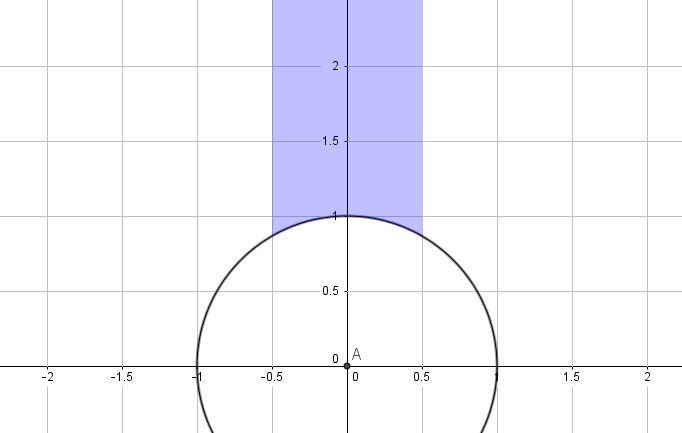
\includegraphics[width=8cm]{lezione-161024-fig3}
\caption{Dominio fondamentale}\label{fig:2}
\end{figure}

Anticipazione: la prossima volta si vedranno gli automorfismo di un reticolo e i gruppi olomorfi, per questi ultimi si darà un cenno al concetto di funzione olomorfa in più variabili.
